\chapter{Theoretical Basics} \label{chapter:basics}
\section{Java}
\subsection{What is Java}
Java is a computing platform and object oriented programming language first released by Sun Microsystems in 1995. Oracle has bought Sun in 2010.\cite{JavaWhat}
\\



The Java platform consists of the Java application programming interfaces (APIs) and the Java virtual machine (JVM).
\\



Java is class-bases and object oriented. It is intended to let application developer's write once, run anywhere' meaning that code that runs on one platform does not need to be recompiled to run on another. Java programs are compiled to byte-code. this code can run on any JVM regardless of the real computer architecture.\cite{javaWiki}
\\

Java is next to C/C++ one of the most popular programming languages.\cite{progLangPop} The language also has a similar syntax to C and C++.

\subsection{Class Based \& Object Oriented}
Class-based object-oriented languages, such as Java , are founded on the concept of two distinct entities: classes and instances.

\begin{enumerate}
\item \textbf{Class:} A class is a blueprint or prototype from which objects are created. \cite{javaOBjectOracle} In class-based languages, you define a class in a separate class definition. In that definition you can specify special methods, called constructors, to create instances of the class. A constructor method can specify initial values for the instance's properties and perform other processing appropriate at creation time.\cite{javaObjectClass} In Java the \textbf{new} Operator is with a call of the constructor method is used to make a new instance of a class. 


\item \textbf{Instance:} An instance or object is the instantiation of a class that is one of its members. Software objects are often used to model the real-world objects

\item \textbf{Interface:} An interface is a collection of empty methods. When a class implements an interface, in java with the keyword \textbf{implements}, it has to implement all methods of the interface. A class describes the attributes and behaviors of an object. An interface contains behaviors that a class implements. 

\item \textbf{Subclasses:} In a class-based language, you create a hierarchy of classes through the class definitions.\cite{javaObjectClass} The subclass, in Java the keyword \textbf{extends} is used, provides all functionalities of the super class an can add new ones ore modify the existing properties.

\begin{figure}[H]
\centering
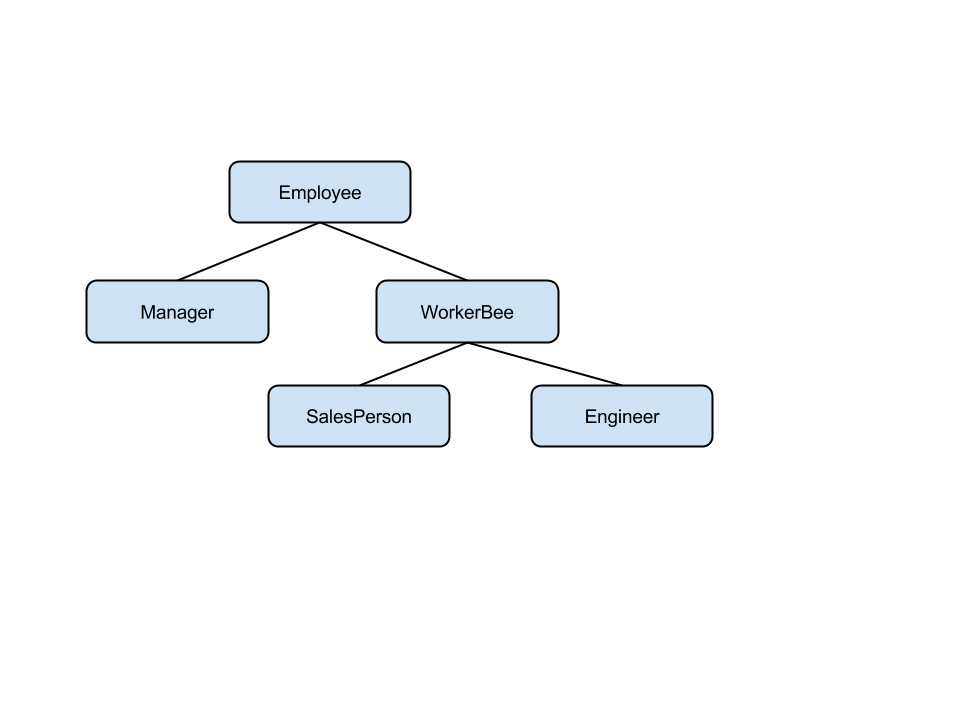
\includegraphics[width=1.0\linewidth]{graphics/java_subclass.PNG}
\caption{Java Subclasses}
\end{figure}
As you can see in this example \textit{Engineer} is an \textit{Employee}. But \textit{Manager} which also is an employee has not the same properties. 


\item \textbf{Abstract Class:}
An abstract class is a class that can't be instantiated. It's only purpose is for other classes to extend. Abstract classes are similar to Interfaces but an abstract class, in contrast, provides more structure. It usually defines some default implementations and provides some tools useful for a full implementation.\cite{javaAbstractVsInterface}

\item \textbf{Package:} 
A package is a namespace for organizing classes and interfaces. Packages make large software projects easier to manage. \cite{javaOBjectOracle}
\end{enumerate}


\subsection{Design Patterns}
Design patterns are proven solutions approaches to specific problems. A design pattern is not a framework! They are based on the base principles of object orientated design. 

\begin{enumerate}
\item Program to an interface not an implementation
\item Favor object composition over inheritance.
\end{enumerate}

\subsection{Performance}
Programs written in Java have the reputation of being slower than other languages. However in the last 10 years the JVM execution speed increased dramatically. In six separate web performance benchmarks, Java frameworks took 22 out of the 24 top-four positions. The JVM has been optimized that much that Java code is now running nearly as fast as C++ code. \cite{javaPerfromance}

\subsection{JVM}
The Java virtual machine is what makes Java a platform independent programming language. A virtual machine (VM) is a software implementation of a machine (i.e. a computer) that executes programs like a physical machine. Therefore, the JVM runs on all kinds of hardware to execute the Java Bytecode without changing the Java execution code. Java developers do not need to know how the JVM exactly works. However a deeper knowledge of the JVM helps understanding how JAVA works and can be helpful to solve various problems.\cite{javaJVM} 
\\


Features of JVM:
\begin{enumerate}
\item \textbf{Stack-based virtual machine:} Most computer architectures such as Intel x86 Architecture and ARM Architecture are based on registers. Whereas the JVM is stack based.\cite{javaJVM} That means that the VM doest need to know the operand addresses, it only calls the Stack-Pointer which points to the current instruction. \cite{stackBased_vs_registerBased} 
\item \textbf{Symbolic reference:} All data types except for primitives are referred to through a symbolic reference.   
\item \textbf{Garbage collection:} The garbage collector frees the memory from objects that are not in use any more. \cite{javaGarbageCollector}  
\item \textbf{Guarantees platform independence by clearly defining the primitive data type:} In other more tradition languages like C or C++ primitive data types have different sizes according to the System. In Java the JVM defines a fixed size for primitives. 
\end{enumerate} \cite{javaJVM}

\subsection{Java bytecode}
The Java bytecode is the result of a compiled Java source-code. It is a middle-language between Java and the machine code. \cite{javaJVM}  

\subsection{Java Code Execution Process} 
The Java code execution process is shown in the figure bellow. 
\begin{figure}[H]
\centering
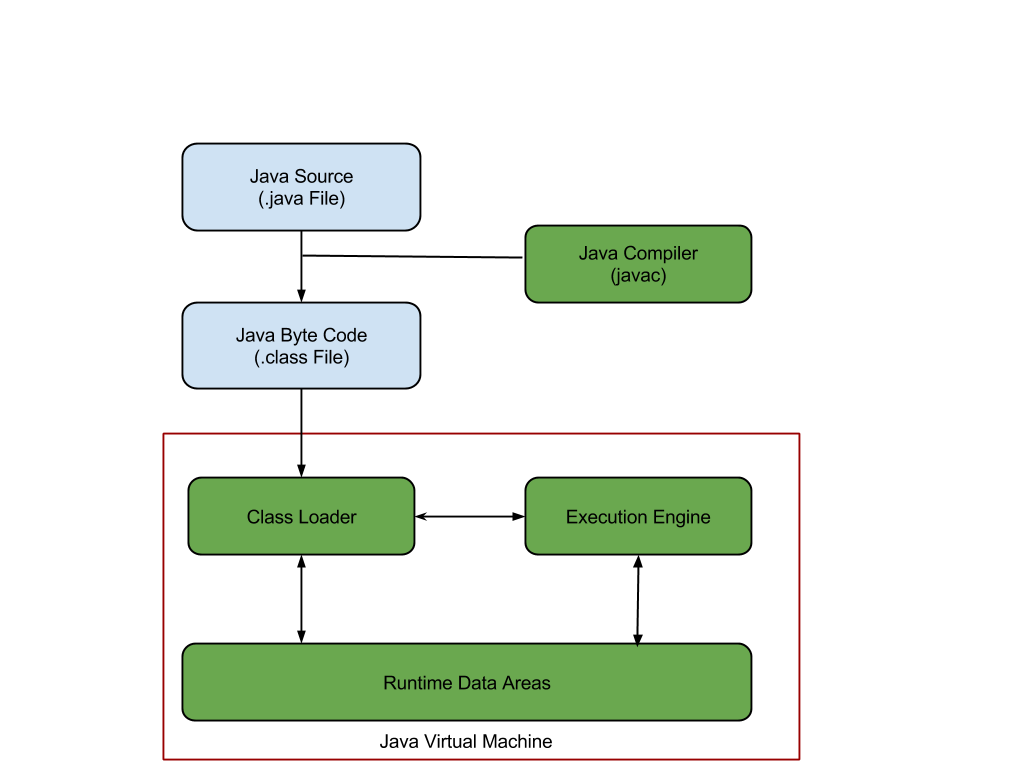
\includegraphics[width=1.0\linewidth]{graphics/java-code-execution-process.png}
\caption{java code execution process}
\end{figure}
\subsubsection{Class Loader}
The Java Class Loader loads and links a class when it refers to a class the first time at runtime. Every class loader has its own namespace that stores the loaded classes.\cite{javaJVM} 

\subsubsection{Runtime Data Areas}
The JVM Runtime Data Areas is the Memory assigned to a program when it runs on the OS. They can be divided into six areas: the Pc Register, JVM Stack, Native Method Stack, Heap, Method Area, and the Runtime Constant Pool. The first three are created for a single thread the other areas are shared by all threads.  

\begin{enumerate}
\item \textbf{PC register:} One \textbf{program counter} register exists for one thread. It gets created when the thread starts. Pc register has the address of the JVM instruction that is executed now.\cite{javaJVM}
 
\item \textbf{JVM Stack:} Each thread has a private JVM Stack, created the same time as the thread. A Java Virtual Machine stack stores frames. Frames are used to store data and results, new frames are created each time a method is invoked. It gets destroyed when its method invocation completes, whether that completion is normal or abrupt (it throws an uncaught exception). \cite{javaVMOracle}

\item \textbf{Native Method Stack:}
A stack for native code written in a other language than Java. It is a stack used to execute C od C++ Methods.\cite{javaJVM}.  

\item \textbf{Heap:}
The JVM Heap is a data area that is shared among all Java Threads. The heap is created on virtual machine start up.
Its a space that stores all class instances Arrays and Variables. If a program requires more heap space than aviable the Java Virtual Machine throws an \textbf{OutOfMemoryError}\cite{javaVMOracle}

\item. \textbf{Method area:} The method area is shared by all threads, created when the JVM starts. It stores runtime constant pool, field and method information, static variable, and method bytecode for each of the classes and interfaces read by the JVM. Unlike in the heap the garbage collection in the method area is optional for each JVM version. \cite{javaJVM}

\item \textbf{Runtime constant pool:}
The Runtime pool is a part of the Native Method stack and gets created when a class or interface gets created. Its the run-time representation of the \textbf{constant pool} table in a class file. This constant pool table contains several constants \cite{javaVMPaper}

For example:
\begin{lstlisting}[language=Java, caption=Java example Code]
System.out.println("Hello, world!");
\end{lstlisting}
Generated byte-code:
\begin{lstlisting}[language=Java, caption= JVM bytecode]
0:   getstatic       #2;               
3:   ldc     #3;                         
5:   invokevirtual   #4; 
\end{lstlisting}
\#n indicates that this is a reference to the constant pool.
2 is a symbolic reference to \textit{System.out}, \#3 is the \textit{Hello, world!} string.\#4 references to the \textit{PrintStream.println(String)} method.
\cite{javaVmstover}  
\end{enumerate}
\begin{figure}[H]
\centering
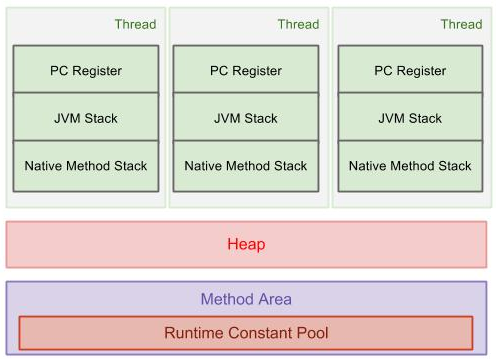
\includegraphics[width=1.0\linewidth]{graphics/java-data-areas.PNG}
\caption{Java Run-time Data Areas}
\end{figure}
\newpage

\subsubsection{Execution Engine}
The bytecode that is assigned to the runtime data areas in the JVM loaded from the class loader is executed by the execution engine. The execution engine reads the Java Bytecode in the unit of instructions. It is like a real CPU executing the machine commands one by one. Each command consists of 1 Operation Code byte and an additional Operand code. The execution engine gets one OpCode and execute task with the Operand, and then executes the next OpCode.\cite{javaJVM}  

\subsection{.JAR File}
A JAR \textbf{(Java ARchive)}is a file  that contains the class, image, sound, etc. files for a Java application or applet gathered into a single file and possibly compressed. \cite{javaJarMargaret}

\subsubsection{Executable JAR }
Its also possible to create a executable .Jar files. It behaves similar to a .exe file in Windows. It can be executed with a double click when Java is installed on the system. 

\section{JavaScript, HTML5,CSS3}
 \subsection{JavaScript}
 Web programing uses JavaScript. It is used to make the web page interactive. JavaScript is very usefull to change the content dynamically of a web page. It is also a expansion for HTML5 and CSS. JavaScript was developed in 1995 by Brendan Erich. JavaScript describes a dynamic typed, object oriented and classless scripting language.\cite{javascript}
 \\\\
 \subsection{HTML5}
 Html5 is the latest standard version of HTML. HTML has also previous version such as HTML 4.01, came in 1999. In 1999 the internet has changed significantly.HTML5 was created to replace  both HTML 4, XHTML and the HTML DOM Level 2. HTML5 is designed such that nobody has to use plugins. It is capable of: animations to graphics, music to movies, and it can also be used to build complicated web applications. The big benefit from HTML5 is ,it being cross-platform. It can be used for designing apps for PC, Tablet, Smartphone and TV.\\\\
 HTML5 is a cooperation between the World Wide Web Consortium (W3C) and the Web Hypertext Application Technology Working Group (WHATWG).\\\\
 
  The new features of HTML5 is to play video and audio in a easier way. The next ability is to draw graphics. With HTML5 , web applications can be developed with helpful elements such as:\\
  \begin{itemize}
  \item Local data storage
  \item Local file access
  \item Local SQL database
  \item Application cache
  \item Javascript workers
  \item XHTMLHttpRequest 2
  
  \end{itemize}
  
  Furthermore HTML5 is able to use CSS3.\cite{html5}
  \\\\
  \subsection{CSS3}
  CSS3 is the latest version of CSS. The benefit of CSS3 is, it is completely backwards-compatible with earlier version of CSS. Moreover CSS3 has been split into 'modules'. However it contains old CSS specification, which has been split into smaller pieces .
  \\\\
  The new Modules that has been added and which are most important in CSS3 are:\\
  \begin{itemize}
  \item	Selectors
  \item	Box Model
  \item Backgrounds and Borders
  \item	Image Values and Replaced Content
  \item	Text Effects
  \item	2D/3D Transformations
  \item	Animations 
  \item 	Multiple Column Layout
  \item User Interfaces
  
  \end{itemize}
  \cite{CSS3}
  \\
  The listed modules are used in this project in combination with jQuery Mobile. JQuery will be described in the following chapter.
  \section{jQuery Mobile}
  jQuery Mobile is touch-optimized web framework. This framework was created by the JQuery Foundation. It is completely open source. This framework is also one of the most popular mobile frameworks. That's the  reason why this project NAVAR uses jQuery Mobile framework. This framework was created by Jasper de Groot, Alexander Schmitz, Anne-Gaelle Colom, Gabriel Schulhof.\\\\
  
  jQuery Mobile is a HTML5 based user interface system, it is designed to create responsive web sites and apps that are accessible on all smartphones, tablets and desktop devices. The framework is build on jQuery and jQuery UI foundation. It offers also AJAX navigation with page transitions, touch events and it has other interesting components and features. This framework is a lightweight code, so it has a flexible ,easily theme able design. \\\\
  
  jQuery Mobile  also updates their framework versions. To built a theme with the framework is not so difficult. The user interface has the components of jQuery Mobile. The components of jQuery will be explained in Chapter Design concept.\\\\
  
  \section {AJAX}
  AJAX (Asynchronous JavaScript and XML) is a method which is widely used in web development. Ajax uses several technologies like: JavaScript, CSS, XML and XMLHttpRequest.\cite{ajax}
  \\
  \subsection{XML}
  \textit{''Extensible Markup Language (XML) is a simple, very flexible text format derived from SGML (ISO 8879). Originally designed to meet the challenges of large-scale electronic publishing, XML is also playing an increasingly important role in the exchange of a wide variety of data on the Web and elsewhere.''}\cite{xml}
  \\
  \subsection{XMLHttpRequest}
  XMLHttpRequest is used in Ajax for exchanging data with a server. The main advantages of this request is that it can be used in the background for sending data to the server, updating a page without reloading it, request and receive data from the server after the page is loaded.\cite{xmlHttp} 
  \newpage
  \subsection{How does AJAX work?}
  \begin{figure}[htbp]
  \centering
  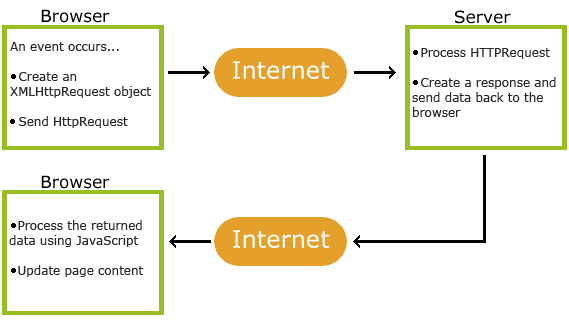
\includegraphics[width=100mm,height=\textheight,keepaspectratio]{graphics/ajaxwork.png}
  \caption{AJAX overview\cite{ajax}}
  \end{figure}
  
  As described in the graphic, whenever a program needs to send data from the browser to the server it creates an XMLHTTPRequest object. This request is then accepted or denied by the server and a response will be sent back to the browser where it can be displayed or processed. 
  
  \section{Windows Azure}
  \textit{''Azure is an open and flexible cloud platform that enables you to quickly build, deploy and manage applications across a global network of Microsoft-managed datacenters. You can build applications using any language, tool or framework. And you can integrate your public cloud applications with your existing IT environment''}\cite{azure}
  \subsection{Overview}
  \begin{figure}[htbp]
  \centering
  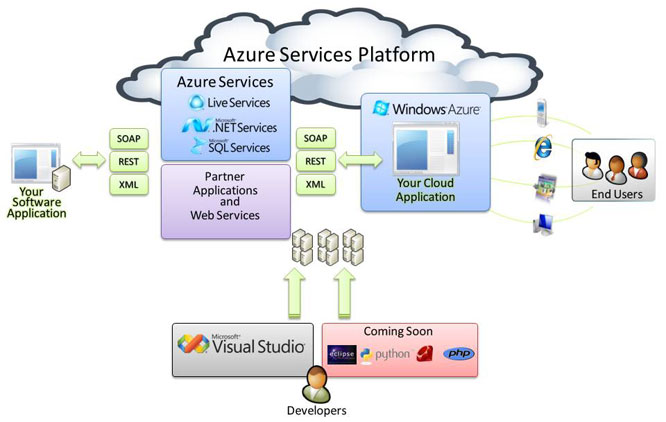
\includegraphics[width=100mm,height=\textheight,keepaspectratio]{graphics/azurePlattform.jpg}
  \caption{Azure overview}\cite{azureOver}
  \end{figure}
  
  The typical Windows Azure environment consists of many components such as the Azure Service Platform, which can be several virtual machines with services. A software application which communicate with Azure over XML and other technologies. Several end users which access the Azure cloud over a browser and developers who access the cloud directly. 
  \newpage
  \section{Microsoft SQL Server}
  Microsoft SQL Server is a relation database software for saving,modifying and providing data. Microsoft SQL Server can be deployed on a desktop server as well as in the cloud.It provides a edition for high-end performanc, critical applications and a lighter version for normal applications/data.\cite{sqlserver}
  \\\\
  There are five main releases of MS SQL Server:
  \begin{itemize}
          \item Microsoft SQL Server 2005
          \item Microsoft SQL Server 2008 
          \item Microsoft SQL Server 2012 
          \item Microsoft SQL Server 2014
  \end{itemize}
        \cite{sqlserver}
  \subsection{Program Overview}
  \begin{figure}[H]
  \centering
  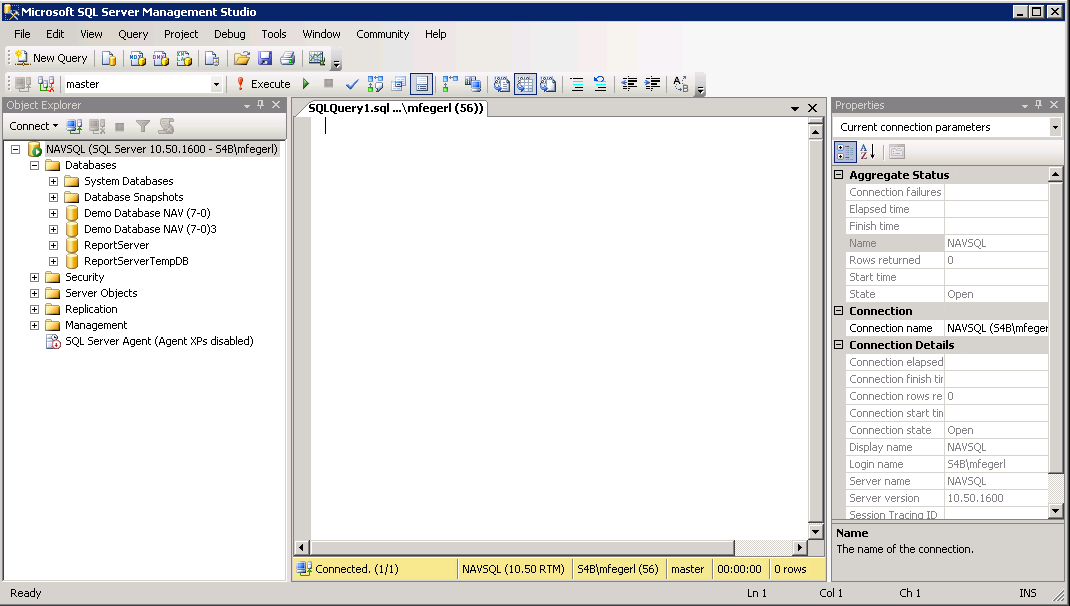
\includegraphics[width=\textwidth,height=\textheight,keepaspectratio]{graphics/sqlserver.PNG}
  \caption{SQl Server 2008 overview}
  \end{figure} 

  The figure shows the graphical user interface of  Microsoft SQL Server Management Studio. It is used to maintain and configure SQL databases. In the left panel of the program the available databases are shown.The panel in the middle is a simple editor for database queries.On the right side the properties of the selected datbase are displayed.    
  \newpage
  \section{Microsoft Dynamics NAV}
  Microsoft Dynamics NAV is an ERP(Enterprise Ressource Planing) software for small and medium sized corporations. It is a highly adaptable software which provides functionalities for managing a whole business. Such as sales, shipping, financing, project management, supply chain management, business intelligence,reporting and other services. 
  The look and feel of the application is based on Microsoft Office to provide a simple entry point to the product if you are familiar with Microsoft Office. Microsoft NAV can be either installed on local servers as a 3-tier ,2-tier or 1-tier implementation as well as in the cloud to provide the best solution for a business.\cite{navOver} 
  
  \subsection{Program Overview}
  The following figure shows the graphical user interface of Microsoft NAV, the RoleTailored client(RTC).It shows the RTC for the role sales manager with the demo Database ''CRONUS International Ltd.'' from Microsoft. 
  \begin{figure}[htbp]
  \centering
  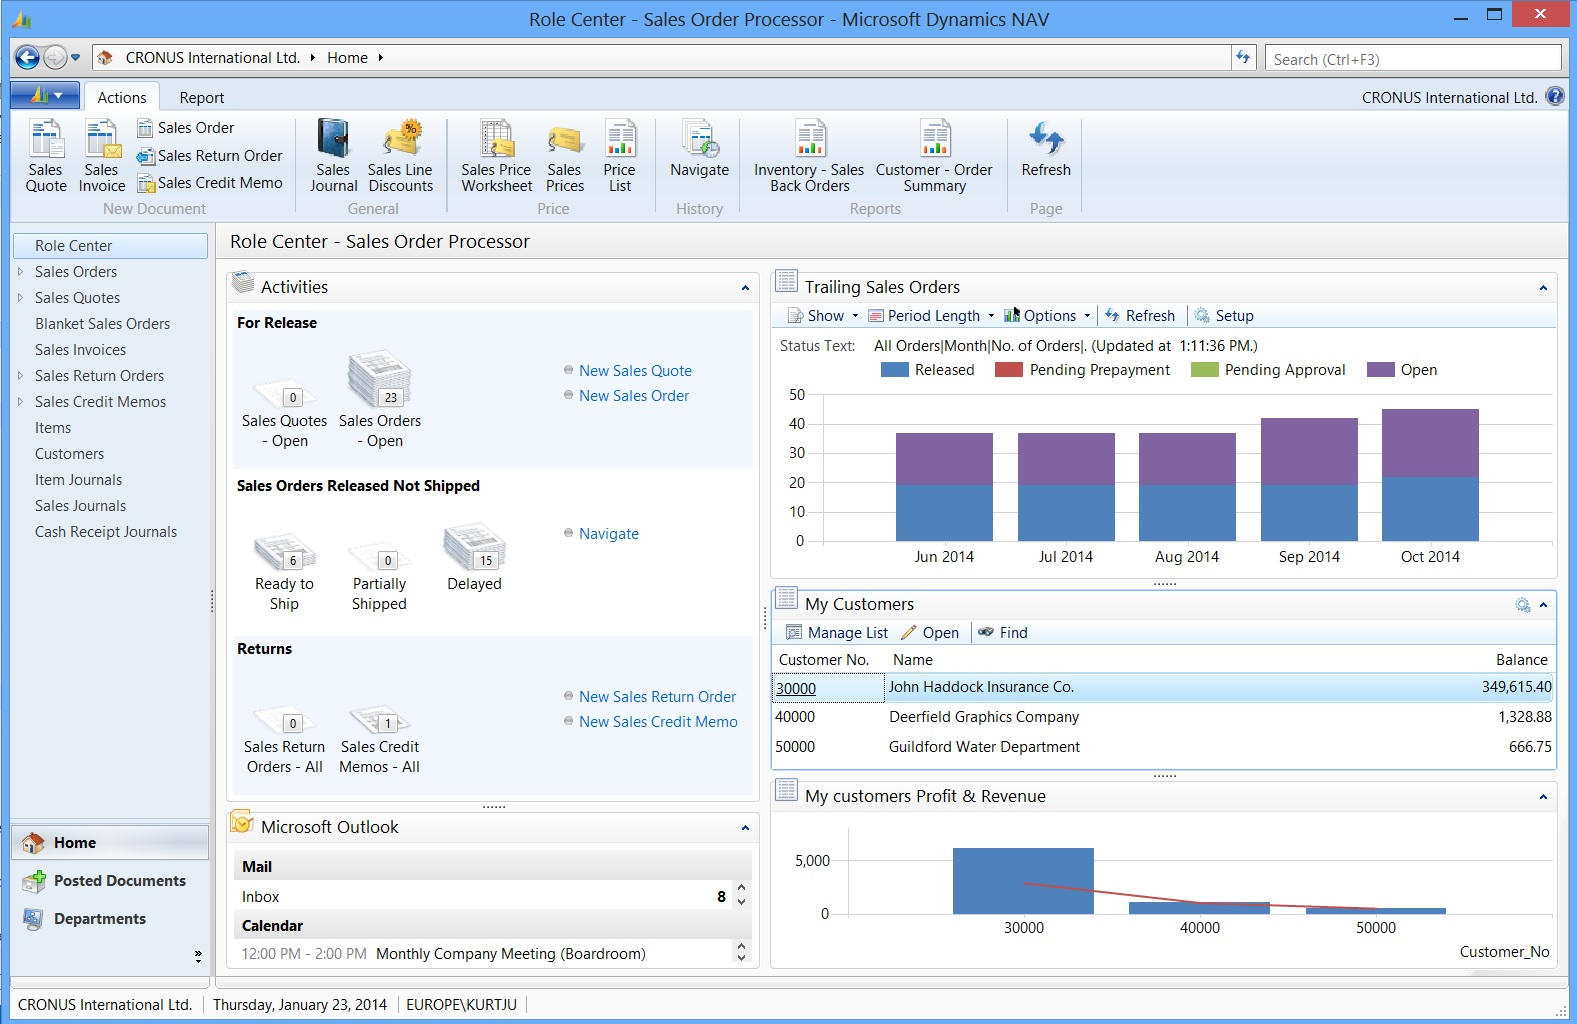
\includegraphics[width=\textwidth,height=\textheight,keepaspectratio]{graphics/navSales.jpg}
  \caption{Program overview}\cite{azureOver}
  \end{figure}
  \newpage
  
  \subsection{Data structure}
  \subsubsection{Tables}
  Microsoft Dynamics NAV saves data into a Microsoft SQL Server database.The databases consist of several tables, which can be created, edited and deleted.\\Table's are the basic modules of the database and are fundamental.It provides the functionality to modify,delete and display data on the run.
  \\\\
  \begin{figure}[htbp]
  \centering
  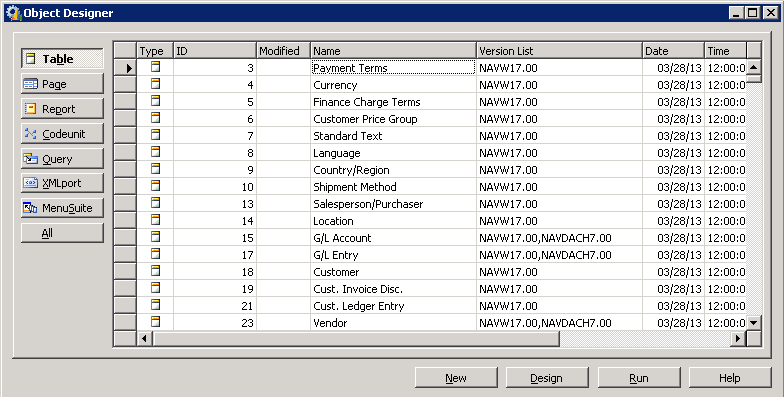
\includegraphics[width=\textwidth,height=\textheight,keepaspectratio]{graphics/navTable.PNG}
  \caption{Table example}
  \end{figure}
  \newpage
  \subsubsection{Pages}
  A page is a XML object which consists of several properties and code. It is used to display, structure and organize data. It can either be accessed via a client and displayed graphically or trough a web service.In this project the pages are used over a web service by the C\# application. The usage of the pages are explained in the chapter ''Streaming''. 
  \\\\
  The following figure shows an example page with a list of customers.
  \begin{figure}[htbp]
  \centering
  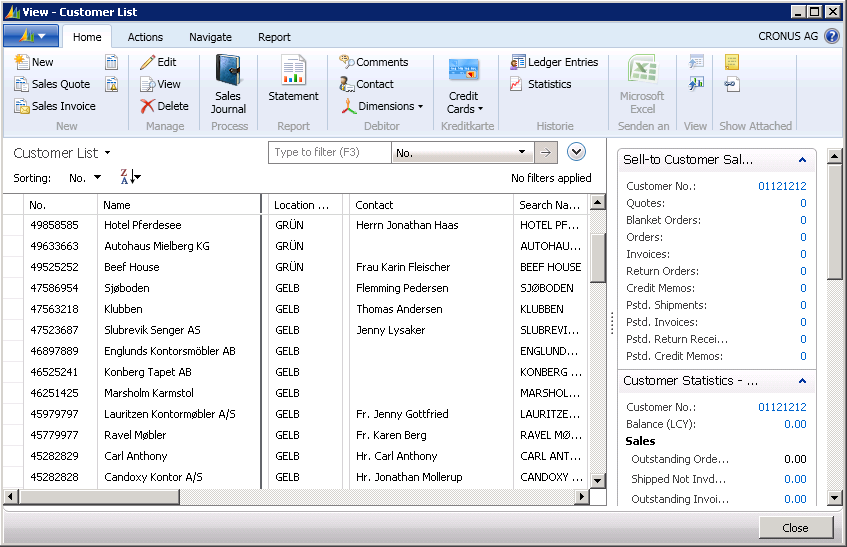
\includegraphics[width=\textwidth,height=\textheight,keepaspectratio]{graphics/customerlist.PNG}
  \caption{customer page example}
  \end{figure}
  \newline
  This page displays the content of the table customers.
  It consist of several attributes such as the name and the telephone number of a specific person.The page provides the functionality to create, delete or  modify the customers within the RTC.    
 
